\documentclass[12pt]{report}

\usepackage[english]{babel}
\usepackage{graphicx}
\usepackage{multirow}
\usepackage[table,xcdraw]{xcolor}

\begin{document}
\begin{center}
    {\Large How does the time it takes a ball to roll down a slope depend on the distance it travels?}

    \vspace{1cm}
    {\large Jason Wells, Kevin Qiao, Stephen Okita and Terri Tai}\newline
    {\large Experiment performed: 20/10/2021}\newline
    {\large Reprt submitted: 26/10/2021}
    \vspace{2cm}
    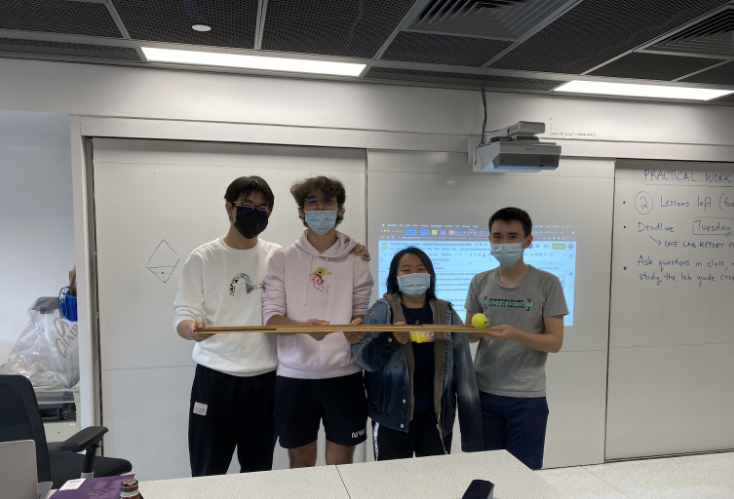
\includegraphics[width=\textwidth]{Img.png}

\end{center}
\tableofcontents
\section{Introduction}
Our experiment attempts to answer the exciting question of How does the time it takes a ball to roll down a slope depend on the distance it travels? Though on the surface this doesn't seem like the most interesting experiment however, with this experiment we get to once again prove the validity of the SUVAT equations and, by extension, Newton's laws of motion. First there are a couple concepts we need to understand the theoretical results.
\begin{figure}
    \centering
    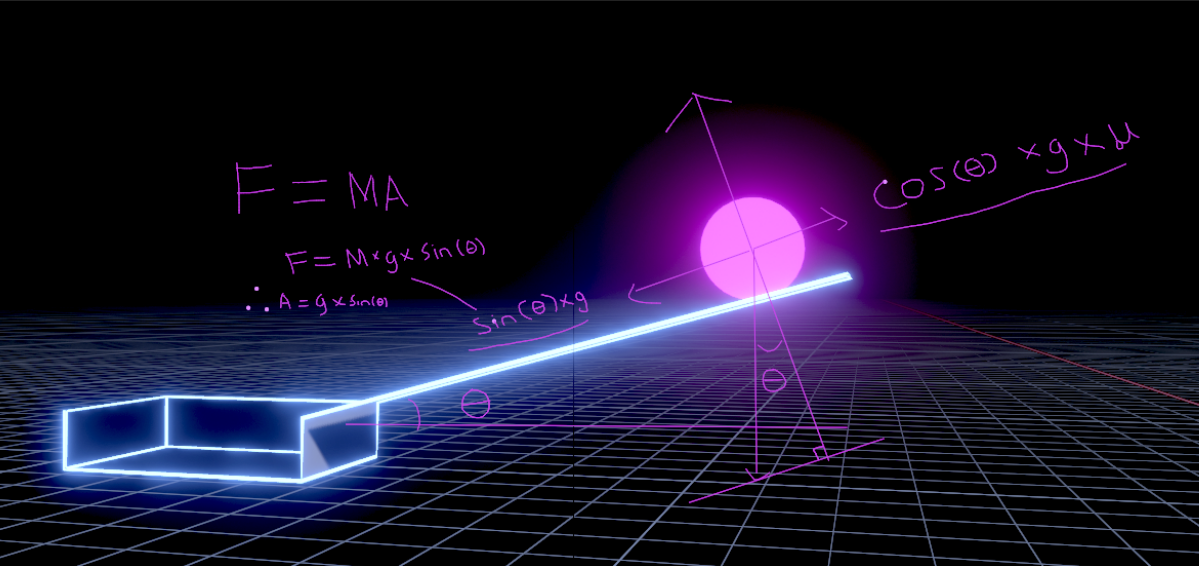
\includegraphics[width=0.5\textwidth]{digram.png}
    \caption{Digram}
\end{figure}

Gravity

On earth gravity at sea level is constant at around 9.8 m/s². This number can be determined through the equation
\[g = \frac{GM}{d^2}\]
This equation shows the acceleration of g is dependent on the total mass of the earth and distance from the centre of the earth.  As we are in Hong Kong, where the gravitational constant is around 9.79 we can just round it to 9.8 as gravity is not the focus of the experiment.

In the diagram above (digram) gravity is expressed by the vector pointing down. Gravity can be decomposed into parallel and perpendicular components. As the ball is on a slope, gravity is no longer solely vertical  so to adjust for the slope we need to multiply the angle we would have to multiply
\[a = g*sin(\theta)\]


Newton's Second law of motion
Once getting the value of g adjusted to the angle, we can use implement it in newtons second law of motion to find the total force exerted by the ball.
Using this we can confirm that acceleration = gravity adjusted for the slope.
\[f = m x g x \sin(\theta)\]
Normal Force
In the diagram above (Image 1) the normal force is represented by the vectors perpendicular upwards to the incline, the normal force cancels out the effect of gravity keeping the ball from falling through the inclined plane, this can be represented by
\[nF = Fg x \cos(\theta)\]
as we have to adjust gravity to the angle of the perpendicular line.

Friction
The friction coefficient is different for each material and is represented by the greek letter mu or µ.
Given the previous information regarding the normal force, we can determine that the friction force is proportional to
\[fF = nF * \mu\]
\therefore
\[fF = m * \cos(\theta) x g x \mu\]

Total acceleration
To find the total acceleration of the ball we need to subtract the Parallel force of gravity by the  Frictional Force which can be represented using this formula,
\[m x g x \sin(\theta)- m *g*\mu*\cos(\theta)\]
By doing some simplification we can get the formula down to
\[a = m(g*\sin(\theta) - g*\mu*\cos(\theta))\]
\therefore
\[a = g(sin(θ) - mu*cos(θ))\] specifically for acceleration.


Suvat Equation

One knowing the total acceleration we can use the suvat equation, the suvat formula’s primary use is to use Newton's second law of motion to determine the values of acceleration, time and initial velocity, using these variables.

S = displacement or the object's total change in position
U = initial velocity
T = Time in seconds
A=  Acceleration
These are expressed through the equation,
\[S = \frac{1}{2}at^2\]
For our experiment the displacement is the independent variable and time is the dependent variable so our final equation would be
\[ y = \sqrt{\frac{2x}{-9.8(\sin(5.17))-0.14\cos(5.17)}}\]
\section{Describing the experiment}
\begin{figure}
    \centering
    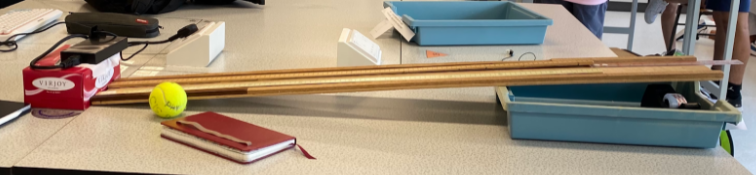
\includegraphics[width=0.5\textwidth]{setup.png}
    \caption{Figure 2: The experiment setup. The red book and tennis ball are to be placed on the ramp when beginning a trial.}
\end{figure}
As seen in figure 2, the setup consists of
\begin{itemize}
    \item A wooden plank with side bumpers
    \item A tray
    \item A tape holder (paperweight)
    \item A tennis ball
    \item A tray with height 7.1cm
    \item A book
    \item A tissue box
    \item A 200w ac-dc adapter for TUF gaming laptop (paperweight)
    \item 2 meter sticks
\end{itemize}
Our experiment was conducted by setting the wooden plank on a sloped angle using the table and the tray, and using materials such as meter sticks, a book, and a tissue box to help control the path of the tennis ball and increase timing accuracy. Paperweights such as the 200w ac-dc adapter for TUF gaming laptop and the tape holder helped keep the setup sturdy.
This is the procedure we followed when conducting the experiment, in numbered order:
\begin{enumerate}
    \item Place the tray on the end of the table and put the tape holder in the tray to prevent it from tilting.
    \item Lay the wooden plank between a short edge of the tray and the table, put the tissue box on the end of the wooden plank opposite the tray, put the 200w ac-dc adapter for TUF gaming laptop on the tissue box to secure it in place, and place 2 meter sticks touching parallel to the side barriers of the wooden plank. Ensure the meter sticks’ 0cm positions sit at the end of the tray, touching the tissue box.
    \item Adjust the position of the tray so that its edge is situated at the 78.8cm mark on the meter sticks. This ensures that the slope of the ramp is kept at a consistent 5.17 degrees angle above from the table, as seen in Figure 3. Note that the tray also needs to be 7.1cm in height.
    \item Place the book vertically on the wooden plank, and place the tennis ball behind the book. The point at which the book and tennis ball touch should be directly above the 100cm mark on either meter stick. Watch out for parallax errors.
    \item Start the stopwatch and immediately remove the book away from the tennis ball, making sure not to apply any additional forces to the tennis ball while doing so. When the tennis ball hits the book, stop the stopwatch. Stopping the stopwatch should be based on predictive timing of when the ball hits the book, not based on reaction time of visual or auditory stimuli.
    \item Repeat steps 4-5 for all remaining trials.
    \item Repeat steps 4-6 for all remaining conditions (90cm, 80cm etc.)
\end{enumerate}
\begin{figure}
    \centering
    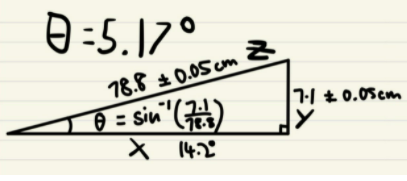
\includegraphics[width=0.5\textwidth]{working.png}
    \caption{Figure 3: a triangle showing measurements for the slope of the ramp, where x is the horizontal distance between the end of the ramp and the tray, y is the height of the tray, and z is the length of the portion of the ramp from its end to its sitting position on the edge of the tray. Theta is the angle of elevation from the table to the ramp.}
\end{figure}
Risk assessment:
Our experiment is quite safe, as we are not dealing with any dangerous equipment. However, caution must be made whilst moving equipment, especially large objects that have pointed edges such as the wooden plank. The tennis ball may also roll on to the floor creating a trip hazard, or it may knock over objects on the table if not kept secured. Ensure that all apparatus is set up exactly as mentioned in the procedure above to minimise the risk of this happening.

Independent variable:
We will be manipulating the distance at which the tennis ball has to roll before reaching the bottom of the ramp. The distance will be measured as the displacement between the point at which the tissue box touches the bottom of the ramp, and the point at which the book touches the tennis ball. For example, if the distance must be 100cm, we would measure 100 cm from the bottom of the ramp using the meter sticks, and place the frontmost end (closest to the bottom of the ramp) of the tennis ball at that location. The book will then be placed in front of the tennis ball so that it stays in place. Our meter sticks are accurate up to ±1mm, however we chose to use 10cm intervals per test to balance accuracy with the time consumption. Distance (x) will be measured and referred to in our results in the unit of centimeters (cm).

Dependent variable:
The dependent variable is the time it takes for the tennis ball to travel a certain distance. The time is measured by a stopwatch, and it’s unit should be second (s). Moreover, we defined time as (t). Due to the fact that the minimum unit of stopwatch is 0.01, the minimum uncertainty of our measurement of time should also be 0.01 seconds.

Controlled variables (MULTIPLE):
\begin{enumerate}
    \item [Mass of the moving object] - We will use the same tennis ball for each trial.
    \item [Level of friction] - We will use the same wooden plank for each trial. This in addition to the controlled tennis ball will guarantee a controlled coefficient of friction between the two materials as the ball rolls down.
    \item [Release force] - No initial velocity will be applied to the ball before it rolls down the ramp. This can be done by quickly removing the book in the same direction that the ball rolls in when conducting each trial.
\end{enumerate}
\section{Data Analysis}
 [Uncertainty of distance:] The meter stick had marks with increments of 0.1 cm, and because it is an analog device, we could estimate that the uncertainty is half of that, which is 0.05. However, we also need to take into account where we stop the ball, which has small errors. There were also errors in where the person released the ball, as they judged it by the human eye. So we estimate an overall uncertainty of around 0.5cm. This is still relatively small in comparison to our variables, with the biggest percentage uncertainty being 5\%.

[Uncertainty of time:] There is uncertainty in the measurement itself as well as human reaction time. We used a stopwatch that had the last digit of 0.01, which is a digital device, therefore the uncertainty is ± 0.01 s. However, we also have to take into account the reaction time of the people who are timing for the experiment, which was Kevin. Hence, he took an examination on this website and his reaction time was on average (around 5 to 6 trials) 295 ms, close to 0.3s, which is much larger than the uncertainty of time. Since the time is determined by the difference between the time in which the tennis ball was released and the time when the ball reaches the bottom of the ramp. So using error propagation, we can put the uncertainty as 0.3 + 0.3 = 0.6 seconds. Nonetheless, we should only take the human reaction time into account for things that are unexpected. Since we counted down to the release of the ball, and we could see the ball approaching the end of the ramp, the random human reaction time cannot be applied for this experiment. Therefore, we decided that taking the standard deviation of the averages was a much better way of estimating the uncertainty.
\begin{table}[]
    \begin{tabular}{ccccccccc}
        \cellcolor[HTML]{6D9EEB}                           & \multicolumn{5}{c}{\cellcolor[HTML]{93C47D}Time} &         &         &                                                                                                                                 \\
        \multirow{-2}{*}{\cellcolor[HTML]{6D9EEB}Distance} & Trial 1                                          & Trial 2 & Trial 3 & Trial 4 & Trial 5 &                           &                                      &                                          \\
        ±0.5cm                                             & ±0.01s                                           & ±0.01s  & ±0.01s  & ±0.01s  & ±0.01s  & \multirow{-3}{*}{Avg} & \multirow{-3}{*}{Sdev} & \multirow{-3}{*}{Unc\%} \\
        100                                                & 2.58                                             & 2.63    & 2.41    & 2.50    & 2.50    & 2.52                      & 0.08                                 & 3.35\%                                   \\
        90                                                 & 2.32                                             & 2.32    & 2.27    & 2.30    & 2.36    & 2.31                      & 0.03                                 & 1.42\%                                   \\
        80                                                 & 1.88                                             & 1.91    & 1.96    & 1.97    & 1.96    & 1.94                      & 0.04                                 & 2.02\%                                   \\
        70                                                 & 1.82                                             & 1.81    & 1.76    & 1.78    & 1.70    & 1.77                      & 0.05                                 & 2.69\%                                   \\
        60                                                 & 1.63                                             & 1.59    & 1.47    & 1.52    & 1.56    & 1.55                      & 0.06                                 & 3.98\%                                   \\
        50                                                 & 1.25                                             & 1.27    & 1.31    & 1.34    & 1.34    & 1.30                      & 0.04                                 & 3.14\%                                   \\
        40                                                 & 1.27                                             & 1.21    & 1.17    & 1.14    & 1.12    & 1.18                      & 0.06                                 & 5.05\%                                   \\
        30                                                 & 1.02                                             & 1.06    & 1.09    & 1.08    & 1.08    & 1.07                      & 0.03                                 & 2.62\%                                   \\
        20                                                 & 0.80                                             & 0.84    & 0.90    & 0.78    & 0.90    & 0.84                      & 0.06                                 & 6.58\%                                   \\
        10                                                 & 0.60                                             & 0.61    & 0.62    & 0.63    & 0.69    & 0.63                      & 0.04                                 & 5.61\%
    \end{tabular}
\end{table}
\caption{Table 1. The raw data from our experiment(here is the link to the spreadsheet). The unit in the first column is all cm and the remaining columns are all in s (as indicated in the headers). The average was calculated by the spreadsheet using the AVERAGE formula and the uncertainty of the average is estimated to be the standard deviation, which was calculated using the STDEV formula.}
\begin{figure}
    \centering
    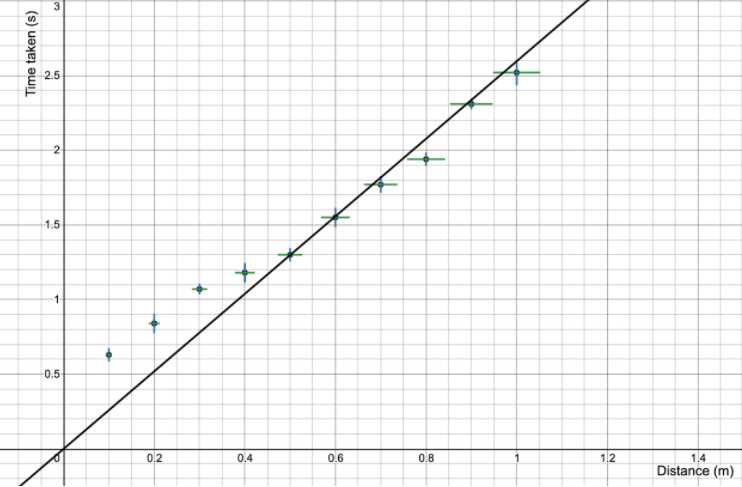
\includegraphics[width=0.5\textwidth]{graph.png}
    \caption{Figure 4. Distance vs. time. Since the straight line through origin does not go through all the windows of uncertainty, it does not accurately depict the relationship between these two variables. }
\end{figure}
We plotted the data into Desmos (in Figure 4). After seeing our data points, we thought that the relationship between the distance and time was a positive linear relationship, where they were directly proportional to each other. We used the best-fit modelling function in Desmos, which gave us the equation 
y=2.60x.This gave us an R^2 of about 0.89, which is the coefficient of determination, which tells us the variability of the data. However, this is not an accurate representation because the graph did not go through all the windows of uncertainty. Additionally, the data was consistently above the model before 0.5 meters, and it fell below the graph after that, showing that the data did not follow a linear trend. Although the R^2 value is quite high, it didn’t make sense overall, so we tried to fit it with another model.
\begin{figure}
    \centering
    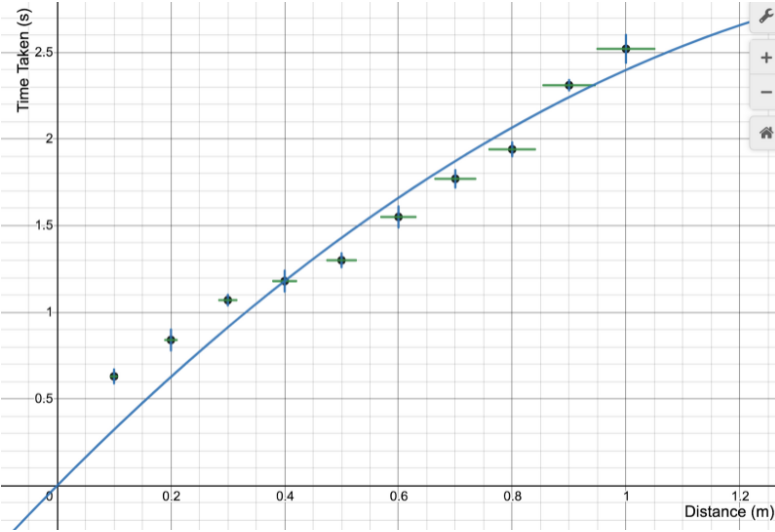
\includegraphics[width=0.5\textwidth]{graph2.png}
    \caption{Figure 5. Distance vs. time. The quadratic equation doesn’t go through all the uncertainties either, meaning this is not an accurate representation of the relationship.  }
\end{figure}
The second model we tried to fit it with is a quadratic model. The equation we got from desmos is \[y = -0.92x^2 + 3.32x\]
where the coefficient of determination is 0.93, which is quite high. However, this is not an accurate representation for a few reasons:
\begin{enumerate}
    \item This graph does not go through all the windows of uncertainty, which means it can not be used to depict the relationship between the distance and the time taken.
    \item This graph implies that the time would decrease after the graph reaches its vertex (at 1.8 meters) and reaches zero again, which doesn't make sense.
\end{enumerate}
\end{Data Analysis}
\section{Conclusion and evaluation}
After sitting down with Mr Mumm, we used the suvat equation \[s = \frac{1}{2}at^2\] to derive a mathematical model. By plugging in our numbers we can get \[s = \frac{1}{2}g(\sin(5.17) - \mu*\cos(5.17)) t^2\], by rearranging the formula to be about time we get the formula \[t =2sg(\sin(5.17)-\mu \cos(5.17))\]. This gives the graph:
\begin{figure}
    \centering
    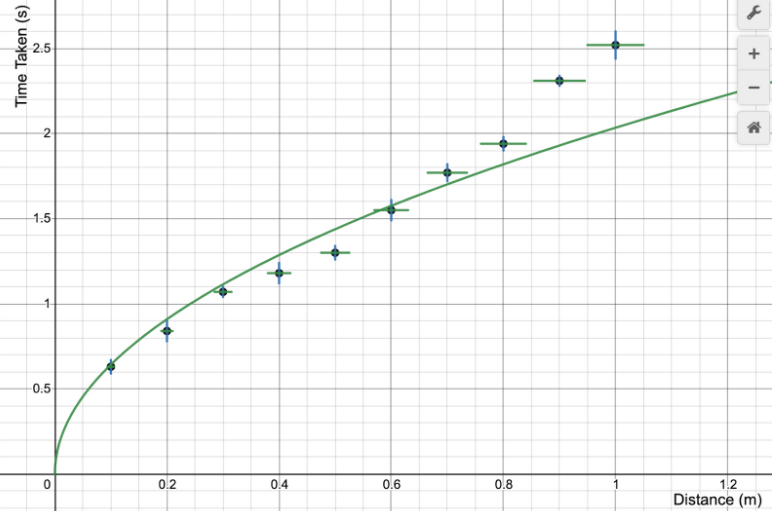
\includegraphics[width=0.5\textwidth]{graph3.png}
\end{figure}
Although this graph does not have the highest coefficient of determination (0.87), and it does not go through all the windows of uncertainty, it’s the model that makes the most sense. The inaccuracy of the graph is most likely due to procedural and random errors, which will be evaluated below.

Evaluation of Procedure:
When we looked back at our procedure, the major problem was the value of the time we measured. We used a long ruler to block the ball at the beginning and a box at the end of the slope to stop it. However, when we lifted the ruler, the ball would remain stationary for a moment because of the wooden slope. A wooden slope has a rough surface, hence, the friction of the ball is relatively bigger than a metal slope, and the angle of our incline was just 5 degrees. Therefore, sometimes the ball stayed still for a short time after the ball was released, but these circumstances did not happen every time. As a result, the time of the ball’s movement would have different values.

Furthermore, the width of the wood slope was huge, when we released the ball, it might not move in a straight line. As we all know, straight lines are shorter than curved lines, which is based on the formula d = st (d: distance, s: speed, t: time) when distance increased, the speed remained constant, the time would increase too. Therefore, in our experiment, the distances that the ball moved in different trails had differences. This phenomenon led to the inaccuracy of our time measurement. There were also bumpers at the side of the slope, which contributed to an increase in friction when the ball hit these bumpers instead of travelling in a straight line. This will also lead to an increase in time taken.

Evaluation of data:
Regarding the data we measured, we calculated the percentage uncertainties for different distances. The lowest value was 1.42\% and the highest was 6.58\%, so the data of our experiment was somewhat precise. The graph we sketched roughly corresponded to our data, but at the beginning and end the curve deviated. The reasons for this were as the longer distance ball travels, it would have more air resistance and friction from the wooden incline plane. Therefore, the time values for longer distances such as 0.8 ~1.0 meters were greater than the curve, and the values of short distance were below the curve.

The function we got for the curve was:
\[ y = \sqrt{\frac{2x}{-9.8(\sin(5.17))-0.14\cos(5.17)}}\]

Moreover, we have the horizontal and vertical uncertainties for the graph were:

\[x = x{1}\{y{1}-z{1}<y<{1}+z{1}\}\]
\[y = y{1}\{0.95x{1}<x<1.05x{1}\}\]
As a result, I believe that the data of the experiment was accurate and precise enough, if we are able to do it again, we will still expect to gain this data.

Conclusion + Expanding on the Project:
In conclusion, after the experiment, the model and data are supporting that when we remain the angle of the inclined plane unchanged, as the release distance increases the time the ball travels also increases. Although the timing and friction of the wood slope would influence the data we received, they didn’t affect the facts in the experiment and the final conclusion.

Furthermore, we are willing to make a new idea of this experiment, which is making the distance the ball travels as a controlled variable and the angle of the inclined plane is an independent variable. The experiment needs people to measure the time the ball travels, and it should be “How does the time it takes a ball to roll down a slope depend on the angle of the inclined plane?”
\section{Bibliography}

\end{document}\